\documentclass{article}

\usepackage{amsmath, amsthm, amssymb, amsfonts}
\usepackage{thmtools}
\usepackage{graphicx}
\usepackage{setspace}
\usepackage{geometry}
\usepackage{float}
\usepackage[hidelinks]{hyperref}
\usepackage[utf8]{inputenc}
\usepackage[spanish,es-nodecimaldot]{babel}
\usepackage{framed}
\usepackage[dvipsnames]{xcolor}
\usepackage{tcolorbox}
\usepackage{tikz}
\usepackage{caption}
\usepackage{longtable}
\usepackage{pdflscape}
\usepackage{svg}
\usepackage{subcaption}
\usepackage{caption}
\usepackage{multirow}
\usepackage{array}
\usepackage{listings}
\usepackage{cancel}
\usepackage{xurl}

\colorlet{LightGray}{White!90!Periwinkle}
\colorlet{LightOrange}{Orange!15}
\colorlet{LightGreen}{Green!15}



\newcommand{\HRule}[1]{\rule{\linewidth}{#1}}

\declaretheoremstyle[name=Theorem,]{thmsty}
\declaretheorem[style=thmsty,numberwithin=section]{theorem}
\tcolorboxenvironment{theorem}{colback=LightGray}

\declaretheoremstyle[name=Proposition,]{prosty}
\declaretheorem[style=prosty,numberlike=theorem]{proposition}
\tcolorboxenvironment{proposition}{colback=LightOrange}

\declaretheoremstyle[name=Principle,]{prcpsty}
\declaretheorem[style=prcpsty,numberlike=theorem]{principle}
\tcolorboxenvironment{principle}{colback=LightGreen}

\newcolumntype{L}[1]{>{\raggedleft\let\newline\\\arraybackslash\hspace{0pt}}m{#1}}
\newcolumntype{C}[1]{>{\centering\let\newline\\\arraybackslash\hspace{0pt}}m{#1}}
\newcolumntype{R}[1]{>{\raggedright\let\newline\\\arraybackslash\hspace{0pt}}m{#1}}

\setstretch{1.2}
\geometry{
    textheight=9in,
    textwidth=5.5in,
    top=1in,
    headheight=12pt,
    headsep=25pt,
    footskip=30pt
}

\lstdefinestyle{bashstyle}{
    language=bash,
    basicstyle=\ttfamily,
    backgroundcolor=\color{gray!10},
    keywordstyle=\color{blue},
    commentstyle=\color{green!40!black},
    stringstyle=\color{red},
    showstringspaces=false,
    numbers=left,
    numberstyle=\tiny\color{gray},
    breaklines=true,
    breakatwhitespace=true,
    frame=tb,
    rulecolor=\color{black!70},
    framerule=0.5pt,
    tabsize=4,
    captionpos=b
}

\lstdefinestyle{javastyle}{
    language=Java,
    basicstyle=\ttfamily,
    backgroundcolor=\color{gray!10},
    keywordstyle=\color{blue},
    commentstyle=\color{green!40!black},
    stringstyle=\color{red},
    showstringspaces=false,
    numbers=left,
    numberstyle=\tiny\color{gray},
    breaklines=true,
    breakatwhitespace=true,
    frame=tb,
    rulecolor=\color{black!70},
    framerule=0.5pt,
    tabsize=4,
    captionpos=b
}

% ------------------------------------------------------------------------------

\begin{document}

% ------------------------------------------------------------------------------
% Cover Page and ToC
% ------------------------------------------------------------------------------

\title{ \normalsize \textsc{}
	\\ [2.0cm]
	\HRule{1.5pt} \\
	\LARGE \textbf{\uppercase{Cambio en los Ingresos de Familias Desplazadas del Meta por el Conflicto Armado}
		\HRule{2.0pt} \\ [0.6cm] \LARGE{Universidad de Bogotá Jorge Tadeo Lozano} \vspace*{10\baselineskip}}
}
\date{}
\author{\textbf{Alvarado Becerra Ludwig} \\
  \textbf{Vera Soto Julián David} \\
	Simulación Estocástica - 20251S}

\maketitle
\thispagestyle{empty}
\newpage

\thispagestyle{empty}
\newpage
\setcounter{page}{1}

Este proyecto es el que se está realizando para la materia de \textit{Autómatas y Agentes} que está cursando uno de los autores, Ludwig Alvarado. Por lo tanto, mucho de la información presente en este documento, ya estaba definida antes de la asignación del presente trabajo.


\section{Descripción del problema}

La migración forzada es un fenómeno que se empeoró a partir de la década de 1990, haciendo que la población afectada se desplace a otras zonas geográficas, generalmente en ciudades urbanas muy diferentes a lo que llevan haciendo toda su vida. Este movimiento incrementa la condiciones de pobreza de los afectados \cite{ruiz2011desplazamiento}. El principal grupo afectado es la población campesina, quienes manejan un modelo de producción agrícola en sus tierras y cuando son forzados a ir a una zona urbana, no pueden adaptarse del todo al modelo agroindustrial que rigen las grandes ciudades del país\cite{bello2003desplazamiento}. Diferentes factores afectan a la economía de los desplazados, sin embargo, no existe una literatura clara para medir el cambio de los ingresos.


\section{Contexto}

La mayoría de campesinos que abandonan sus hogares es por problemas asociados con el conflicto armado. En 1997 el Estado Colombiano reconoce el éxodo forzado como una problemática que exige acciones de política pública enfocadas en la necesidad de prevenir el fenómeno\cite{villa2006desplazamiento}. A pesar de que ya hay leyes para la atención de la población desplazada, los números no han mostrado muchos resultados. A día de hoy hay $9.882.219$ víctimas identificadas\cite{unidadvictimas_ruv_2025}, corresponde cerca del $16,83 \%$ de la población total del país\cite{eswiki:165709323} y supera la población estimada de Bogotá en 2023\cite{eswiki:165573820}. A partir del año 1985 el departamento del Meta ha tenido un incremento de víctimas por el desplazamiento forzado debido a la presencia de diferentes grupos armados\cite{solano2020determinantes}.


\section{Estado del arte}

El desplazamiento forzado se puede categorizar como un fenómeno migratorio, es decir, en la diferente literatura se aplican modelos de migración pero con modificaciones para este tipo de contextos. Se analizó literatura para el conflicto armado en Áfica, donde la literatura en inglés es mucho más abundante y los casos de estudio son mayores. También, se toman casos de estudio a nivel nacional, detallando los modelos que se utilizan y sobre qué se fundamentan. 

% La tesis \textit{Predicting forced displacement using a generalised and automated agentbased simulation}\cite{suleimenova2020predicting} aplica una simulación basada en agentes para predecir el desplazamiento de personas desplazadas en Burundi, República Centroafricana y Malí. Los migrantes seleccionan el lugar de destino utilizando una función de peso de probabilidad que se calcula con ayuda del \textit{atractivo} que tiene un nuevo lugar para el migrante.

El artículo \textit{An Agent - Based Model to Identify Migration Pathways of Refugees: The Case of Syria}\cite{hebert2017agent} utiliza un modelo determinístico para que la población tome una decisión de irse cuando se supere un nivel de tolerancia a la violencia ejercida por el grupo armado. En el artículo cada individuo de la población afectada tiene un nivel de tolerancia a la violencia que se inicializa aleatoriamente y cuando el nivel de violencia ejercido por el grupo armado supera el nivel de tolerancia del individuo, entonces, este toma la decisión de ser migrante. El modelo utiliza varios condicionales para que el campesino decida a qué lugar geográfico irse como se ve en la figura \ref{fig:fig1}. Solamente se contempla este nivel de tolerancia del campesino inicializado aleatoriamente.

\begin{figure}[ht]
  \centering
  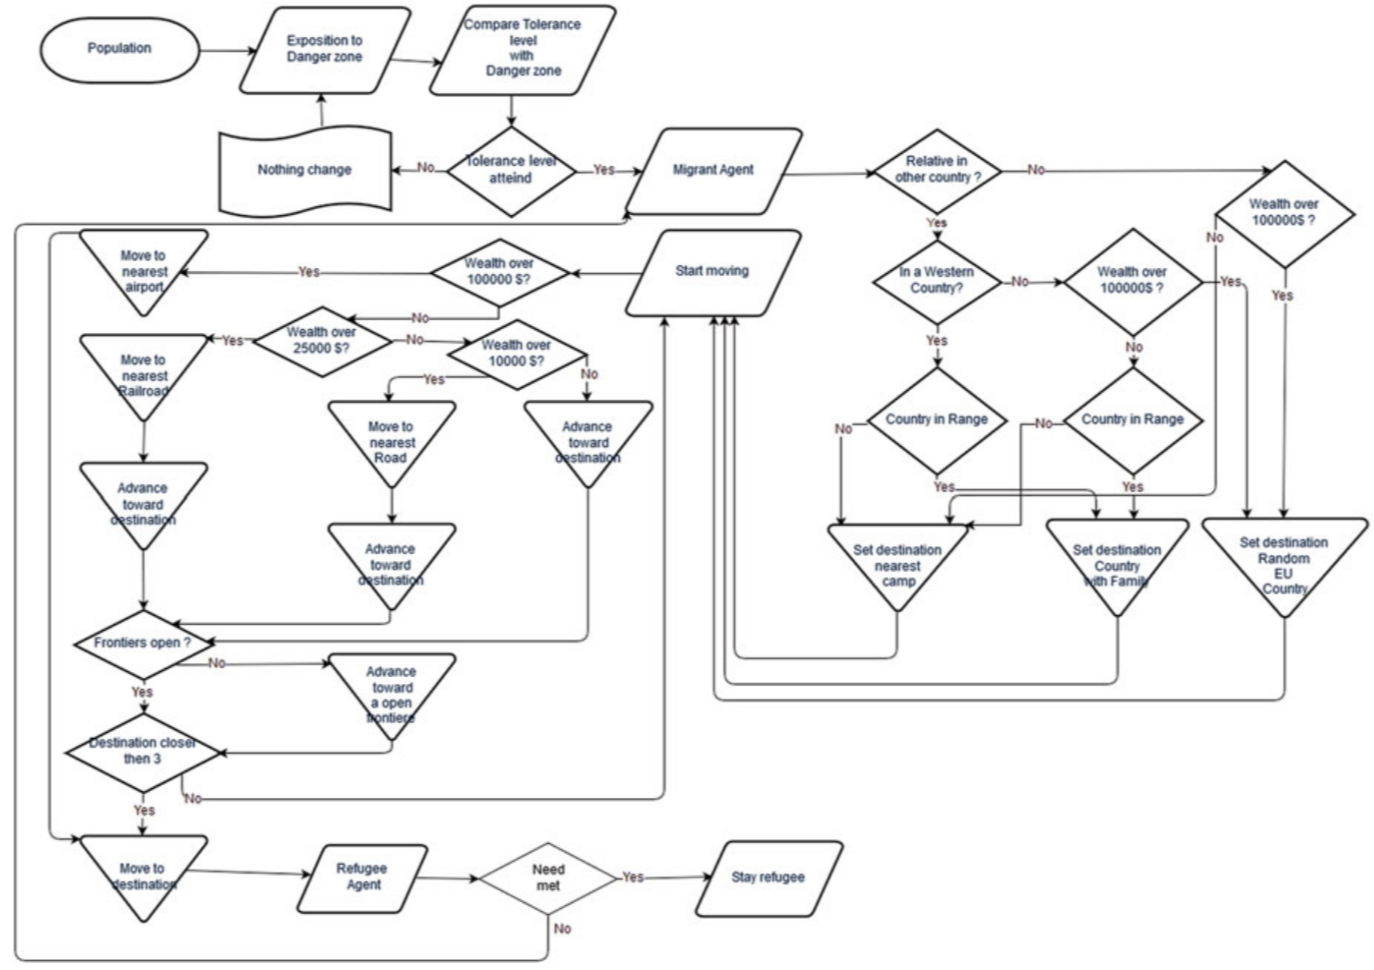
\includegraphics[width=0.5\textwidth]{img/Fig1.png}
  \caption{\label{fig:fig1} Diagrama de flujo para la decisión de a dónde migrar para el campesino.}
\end{figure}


En la tesis de maestría \textit{Teoría de la migración colectiva como explicación al desplazamiento forzado en Colombia}\cite{Gutierrez2012} se propone un modelo de migración en manada aplicada al conflicto armado, es decir, si varios campesinos siguen una trayectoria, un campesino como individuo tiende a seguir esta trayectoria. Se toma en cuenta un parámetro $\omega$ entre 0 y 1 que entre más cercano a 1 el agente no sigue a la mayoría de individuos y entre más cercano a 0 el individuo sigue al grupo. Por otra parte, Pérez \cite{perez2016impacto} utiliza modelos lineales para estimar las cantidades de producción agrícola de los campesinos y cómo estas se ven afectadas al ingresar un grupo armado.





\section{Objetivo general}

Simular el cambio del ingreso económico de la producción agrícola por campesinos del municipio de Meta afectados por el conflicto armado. 


\section{Metodología}

Se va a emplear una simulación basada en agentes con el ambiente programable orientado a agentes \textit{NetLogo}\cite{wilensky1999netlogo}, esto debido a todas las facilidades que posee el lenguaje para utilizarse en estos contextos de agentes. Se van a tener dos agentes principales; grupo armado y campesino. Utilizando programación orientada a objetos se crean dos clases que son los respectivos agentes. La clase campesino tiene atributos como; \texttt{tolerance\_level}, que se inicializa estocásticamente y es el valor de violencia que puede soportar el campesino; \texttt{total\_money}, cantidad de dinero que posee el campesino; y \texttt{migrant}, este es un atributo booleano que muestra si el campesino es desplazado o no. Por otra parte, se contemplan \textbf{atributos} para la generación de dinero de los campesinos. Se va a asumir que todos los campesinos producen los mismos productos y la misma cantidad de unidades. Es decir, el atributo ingreso en cada instante de tiempo $I(t)$ va a ser asignado como:

\[
I(t) = A(t) + B(t) + \cdots + G(t) + \alpha
\]

Donde $A(t), B(t), \cdots$ son los métodos del campesino para producir ganancia a través de sus producciones agrícolas, $G(t)<0$ es lo que el grupo armado le quita al campesino, y $\alpha$ es una variable aleatoria que aún falta por profundizar, aunque se está pensando en utilizar series de tiempo, sin embargo, el conocimiento de los autores en este tema aún se está expandiendo, se espera que en el desarrollo del curso se pueda profundizar esta variable $\alpha$.

Por otra parte, la clase \texttt{GrupoArmado} va a tener únicamente el método $G(t)$ encargado de restar las ganancias de los campesinos.

Las fuentes de datos para la producción de productos agrícolas se toma de la Evaluación de Valoración Ambiental del Departamento Nacional de Planeación de Colombia\cite{EVA2020}. La simulación va a ser iterada durante un (1) año ($t = 1, \dots, 365$). Se espera obtener un gráfico de barras que muestre la cantidad de campesinos que tienen ciertos intervalos de ingresos totales, algo similar a una de las gráficas de la simulación \textit{Simple Economy} encontrada en \url{https://netlogoweb.org/launch#https://netlogoweb.org/assets/modelslib/IABM%20Textbook/chapter%202/Simple%20Economy.nlogo} y que la distribución de riqueza se ve tal como se ve en la figura \ref{fig:fig2}. 

\begin{figure}[ht]
  \centering
  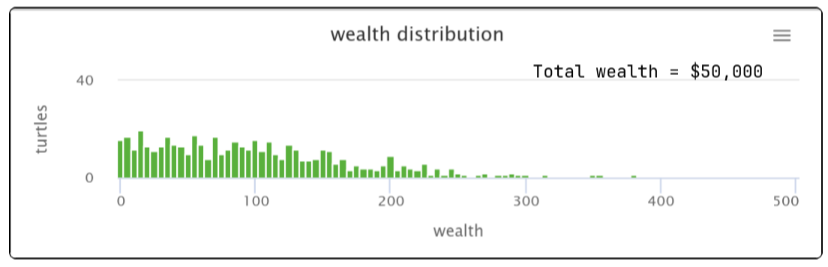
\includegraphics[width=0.7\textwidth]{img/Fig2.png}
  \caption{\label{fig:fig2} Distribución de la riqueza en un modelo económico simple, tomado de \textit{NetLogo Simple Economy model}\cite{wilensky2011simpleeconomy}.}
\end{figure}


No hay manera posible de validar el cambio en la economía de los campesinos, ya que, se vio en la revisión de la literatura que, se afirma sobre que existe un cambio negativo en los ingresos de los campesinos desplazados \cite{perez2016impacto,santacoloma2015importancia,ruiz2011desplazamiento,solano2020determinantes}, mas no cómo se distribuyen los ingresos de esta población. La única manera de validación sería realizar una comparación con el modelo en el tiempo $t = 1$ y $t = 365$, si se observa un descenso en los ingresos, entonces se podría decir que el modelo está en lo correcto, sin embargo, se contemplan más maneras de validar los resultados.


\bibliographystyle{ieeetr}
\bibliography{referencias}





\end{document}
